\documentclass{libs/suep_format}
\usepackage{hologo}
\usepackage[normalem]{ulem}
\usepackage{fontawesome5}
\usepackage{minted}
\usepackage{tipa}
\usepackage{tikz}
\usetikzlibrary{positioning, arrows, shapes, shapes.multipart, backgrounds, calc, automata}
\usepackage{algorithm2e}
\graphicspath{{figures}}

\def\rawcmd#1{\texttt{\color{DarkBlue}\footnotesize #1}}
\def\cmd#1{\texttt{\color{DarkBlue}\footnotesize $\backslash$#1}}
\def\env#1{\texttt{\color{DarkBlue}\footnotesize #1}}
\def\cmdxmp#1#2#3{\small{\texttt{\color{DarkBlue}$\backslash$#1}\{#2\}\hspace{1em}\\ $\Rightarrow$\hspace{1em} {#3}\par\vskip1em}}
\newcommand\pkg[1]{\texttt{#1}}
\newcommand\link[1]{\href{#1}{\faLink}}
\setbeamersize{description width=3em}
\newcommand{\nologo}{\setbeamertemplate{logo}{}}


% Inserting the preamble file with the packages
%%%%%%%%%%%%%%%%%%%%%%%%%%%%%%%%%%%%%%%%%%%%%%%%%%%%%%%%%%%%%%%%%%%%%
%% This file contains the packages that can be used in the beamer. %%
%%%%%%%%%%%%%%%%%%%%%%%%%%%%%%%%%%%%%%%%%%%%%%%%%%%%%%%%%%%%%%%%%%%%%
% Package to fonts family
\usepackage[T1]{fontenc}
% Package to accentuation
\usepackage[utf8]{inputenc}
% Package to Portuguese language
\usepackage[english]{babel}
% Package to Figures
\usepackage{graphicx}
% Package to the colors
\usepackage{color}
% Package to the colors
\usepackage{xcolor}
% Packages to math symbols and expressions
\usepackage{amsmath}
\usepackage{unicode-math}
% Package to multiple lines and columns in table
\usepackage{multirow, array} 
% Package to create pseudo-code
% For more detail of this package: http://linorg.usp.br/CTAN/macros/latex/contrib/algorithm2e/doc/algorithm2e.pdf
\usepackage{algorithm2e}
% Package to insert code
\usepackage{listings} 
\usepackage{keyval}
% Package to justify text
\usepackage[document]{ragged2e}
% Package to manage the bibliography
\usepackage[backend=biber, style=numeric, sorting=none]{biblatex}
% Package to facilities quotations
\usepackage{csquotes}
% Package to use multicols
\usepackage{multicol}
\usepackage{minted}
\usepackage{xeCJKfntef}

% Inserting the references file
\addbibresource{references.bib}

\usefonttheme{serif,professionalfonts}

\lstdefinestyle{style@inline}{
  basicstyle   = \ttfamily,
  keepspaces   = true
}
\lstMakeShortInline[style=style@inline]|

% Title
\title[\LaTeX{} 从入门到入门]{\huge \textbf{\LaTeX{} 从入门到入门}}
% Subtitle
% \subtitle{Subtitle of the Presentation}
% Author of the presentation
\author[数理学院数学系]{纸上得来终觉浅团队}

% Institute's Name
\institute[上海电力大学]{
    \normalsize
    上海电力大学
}
% date of the presentation
\date{\today}


\newcommand\XeTeX{\hologo{XeTeX}}
\newcommand\pdfTeX{\hologo{pdfTeX}}
\newcommand\LuaTeX{\hologo{LuaTeX}}
\newcommand\XeLaTeX{\hologo{Xe}\kern-.13em\LaTeX{}}
\newcommand\pdfLaTeX{pdf\LaTeX{}}
\newcommand\LuaLaTeX{Lua\LaTeX{}}
\newcommand\BibTeX{\hologo{BibTeX}}

\def\texlive{\TeX \ Live}
\def\TL{\texlive}
\def\mactex{Mac\TeX}
\def\BibTeX{Bib\TeX}
% \def\ThuThesis{ThuThesis}
\def\XeLaTeX{\hologo{Xe}\kern-.13em\LaTeX}
\def\pdfLaTeX{pdf\LaTeX}

%%%%%%%%%%%%%%%%%%%%%%%%%%%%%%%%%%%%%%%%%%%%%%%%%%%%%%%%%%%%%%%%%%%%%%%%%%%%%%%%%%
%% Start Document of the Presentation                                           %%               
%%%%%%%%%%%%%%%%%%%%%%%%%%%%%%%%%%%%%%%%%%%%%%%%%%%%%%%%%%%%%%%%%%%%%%%%%%%%%%%%%%
\begin{document}
% insert the code style
\input{libs/code_style}

%% ---------------------------------------------------------------------------
% First frame (with tile, subtitle, ...)
% \begin{frame}{}
%     %% Putting the background image in the frames
%     \usebackgroundtemplate{\includegraphics[width=1.7\paperwidth]{libs/LOGO transparent.png}}
%     \maketitle
% \end{frame}


\setbeamertemplate{background}{
\includegraphics[width=\paperwidth]{figures/background.png}}
\begin{frame}
\maketitle
\end{frame}


%% ---------------------------------------------------------------------------
% Second frame
\begin{frame}{目录}
    \begin{multicols}{2}
        \tableofcontents
    \end{multicols}
\end{frame}

\section{介绍}

\begin{frame}{先声夺人}
  \centering
  \scalebox{5}{\textipa{/"leItEk/}}
\end{frame}

\begin{frame}{\LaTeX{} 是什么?\mbox{}——\mbox{}你为什么学}
\pause
\begin{itemize}
  \item<+-> Word 替代品?

    \begin{itemize}
      \item 「我受够了,我以后什么都要用 \LaTeX{} 写」
    \end{itemize}

  \item<+-> 写论文神器?

    \begin{itemize}
      \item 「我就是为大 paper 而生的,当然必须学 \LaTeX{} 啦」
    \end{itemize}

  \item<+-> 打公式方便?

    \begin{itemize}
      \item 「复杂公式输入哪家强,当然首选 \LaTeX{} 帮忙」
    \end{itemize}
\end{itemize}
\end{frame}


\begin{frame}[fragile]
\frametitle{\LaTeX{} 是什么?\mbox{}——\mbox{}What you \emph{think} is what you get!}
\begin{columns}
\begin{column}{0.48\textwidth}
  \centering
  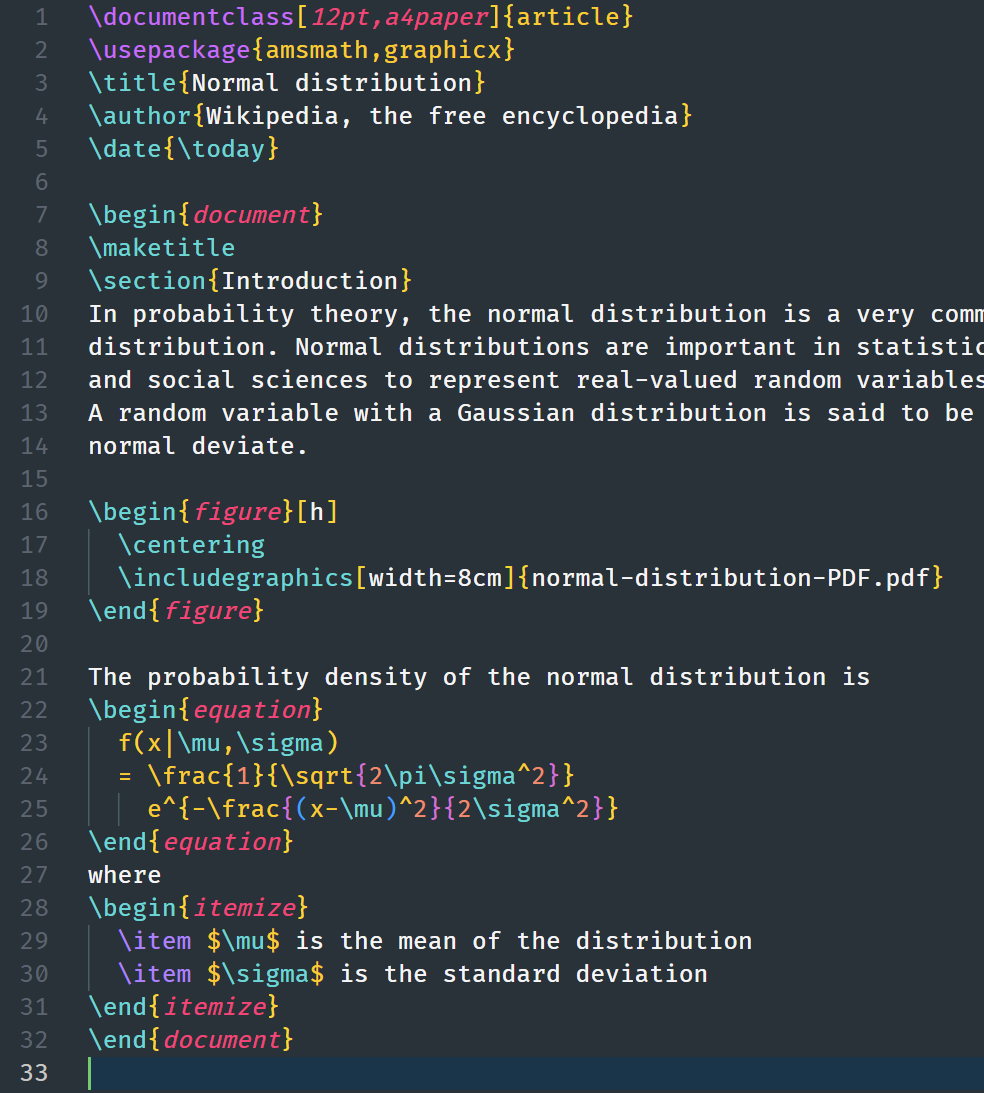
\includegraphics[width=0.75\textwidth]{examples/normal-dist/code.png}
\end{column}
\begin{column}{0.48\textwidth}
  \begin{figure}
    \centering
    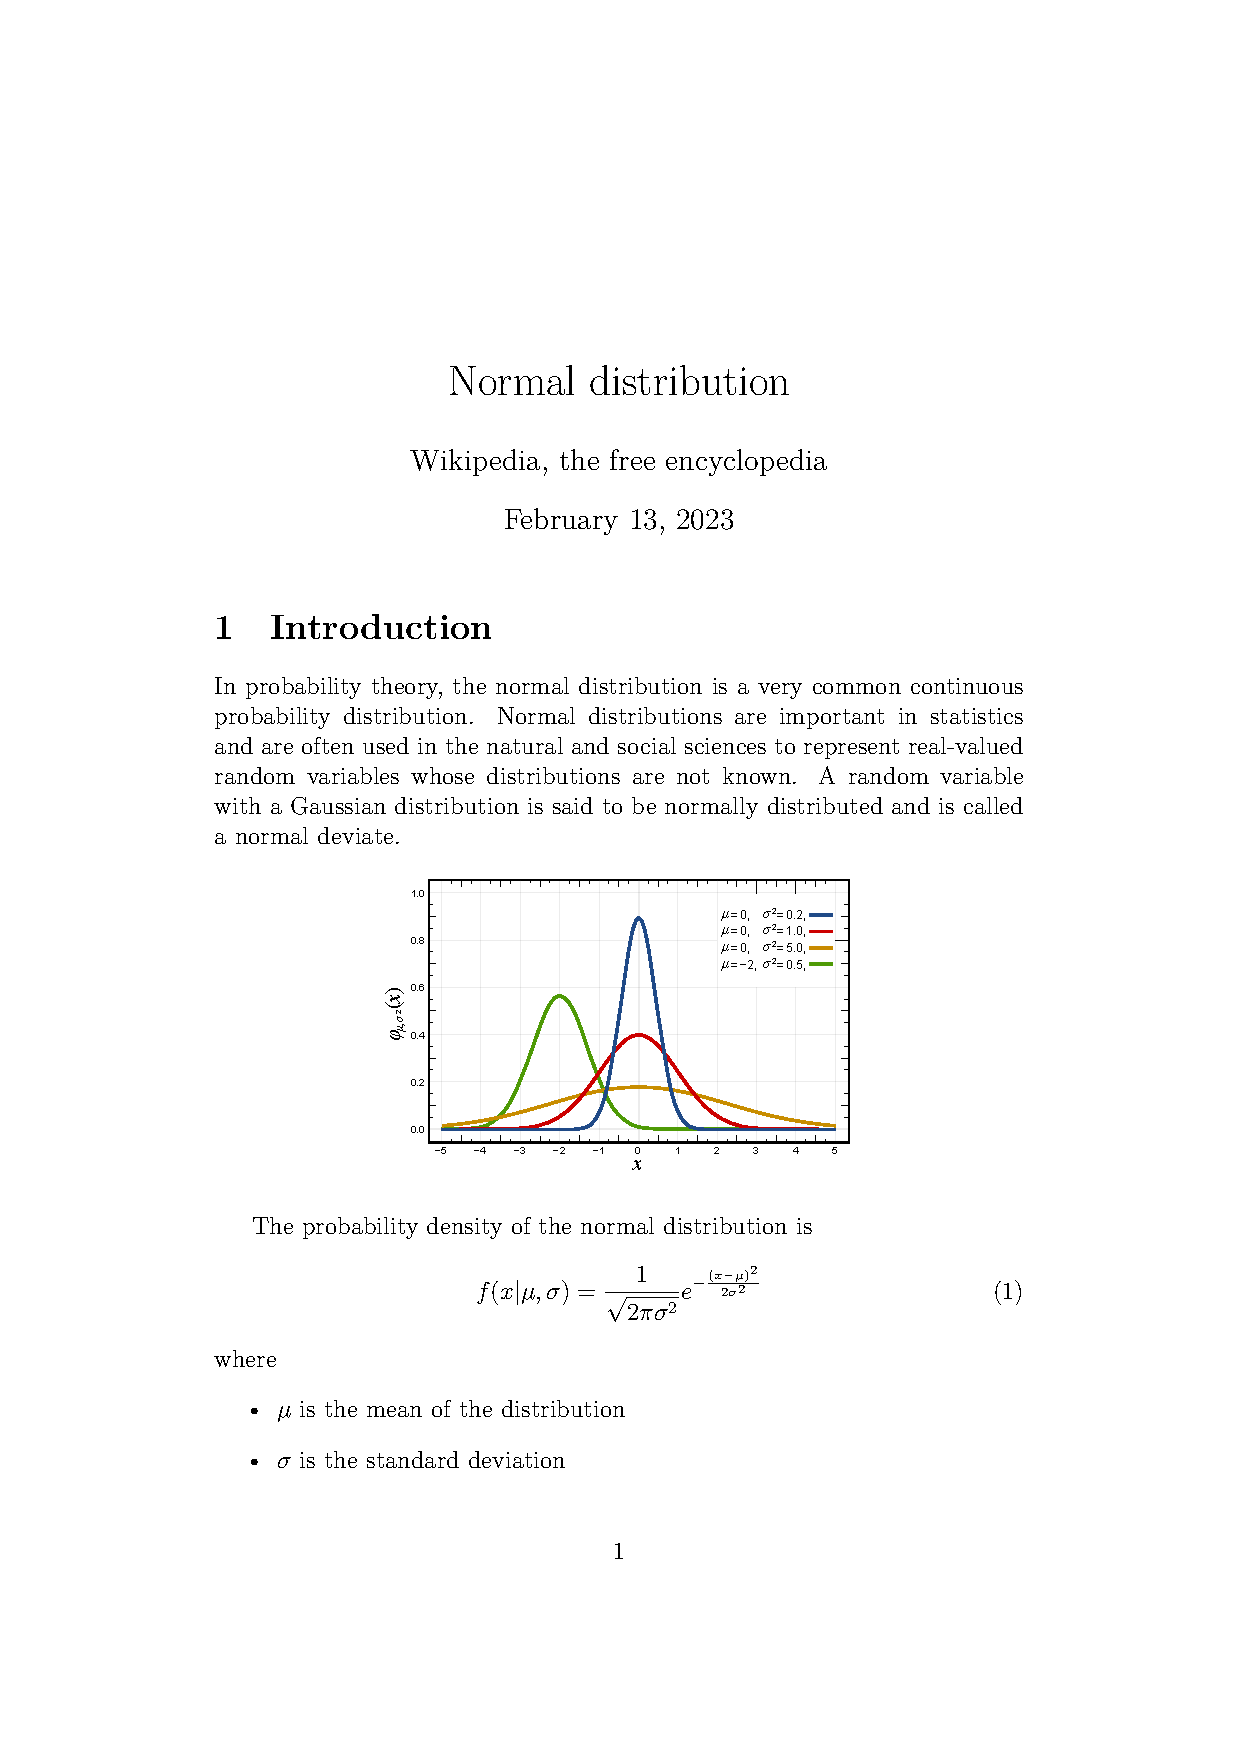
\includegraphics[width=0.75\textwidth]{examples/normal-dist/normal-dist.pdf}
  \end{figure}
\end{column}
\end{columns}
\end{frame}

\begin{frame}{基本原则}
\begin{itemize}
  \item<+-> 排版 vs 文字处理

    \begin{itemize}
      \item 《别把 \LaTeX{} 当 Word 用》
      \item {\scriptsize 在固定版面内,摆置各种不同类型的资料,以最合适的方法呈现 \href{https://zh.wikipedia.org/wiki/排版}{\faWikipediaW}}
    \end{itemize}

  \item<+-> 遵循业界规范
  \item<+-> 追求良好的阅读体验 (readability)
  \item<+-> 内容与格式分离
  \item<+-> \alert{内容永远比格式重要!}
\end{itemize}
\end{frame}

\section{介绍}

\subsection{\TeX 排版系统历史}

\begin{frame}[fragile]{\TeX 与 \LaTeX{} 的起源}
  \begin{columns}[T]
    \column{.7\textwidth}
    \begin{itemize}
      \item \TeX: $\tau\varepsilon\chi$ (\textipa{/'tEx/},
        \textipa{/'tEk/})
        \begin{itemize}
          \item 生成精美图书的排版系统
          \item 最初由 高德纳\footnote{1974年图灵奖得主,《计算机程序设计艺术》(The Art of Computer Programming)作者。} (Donald E.~Knuth) 于 1978 年开发  
          \item 最新版本为 \TeX\ 3.14159265
          \item 漂亮、美观、稳定、通用
          \item 尤其擅长数学公式排版
        \end{itemize}

        \vspace{2em}
      \item \LaTeX{}(\textipa{/'la:tEx/}, \textipa{/'leItEk/})
        \begin{itemize}
          \item Leslie Lamport\footnote{2013年图灵奖得主,对于分布式及并形系统的理论与实践具有基础性贡献。} 开发的一种 \TeX 格式
          \item 在 \TeX 的基础上提供宏包, 降低使用门槛
          \item 极其丰富的宏包,提供扩展功能
          \item 广泛用于学术界,期刊会议论文模板
        \end{itemize}
    \end{itemize}
    \column{.2\textwidth}
    \vspace*{-5mm}
    \hspace{-10mm} 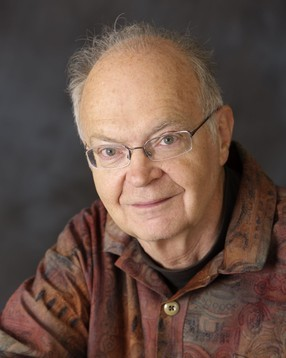
\includegraphics[width=\textwidth]{Knuth.jpg}

    % \vspace*{5mm}
    \hspace{-10mm} 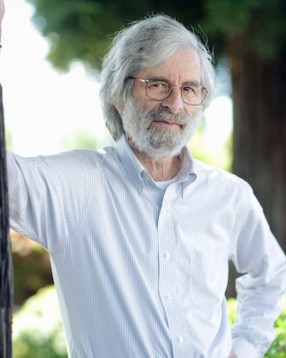
\includegraphics[width=\textwidth]{Lamport.jpg}

  \end{columns}
\end{frame}

\subsection{\LaTeX{} 利弊}

\begin{frame}[fragile]{\LaTeX{} 的好处与坏处}
    \textbf{好处}
    \begin{itemize}
        \item 数学公式排版优雅 \quad $\mathcal{F}(\xi)=\int_{-\infty}^{\infty} f(x)\mathrm{e}^{-\mathrm{j}2\pi \xi x}\,\mathrm{d}x$
        \item 内容与格式分离
        \item 随心所欲的宏定义与自定义命令 \rawcmd{\textbackslash newcommand},\rawcmd{\textbackslash def}
    \end{itemize}

    \vspace{2em}
    \textbf{坏处}
    \begin{itemize}
        \item 得到易读的版本,需要编译
        \item 输入相对 Word 繁琐
        \item 非开箱即用。有时自行解决编辑器、宏包,甚至是编译错误。
    \end{itemize}

\end{frame}

\section{安装}

\begin{frame}{懒得折腾?}
    \begin{itemize}
    \item 云端服务可能更好用
    \item 免去安装、升级等一系列烦恼,可以多人协作
    \item 版本管理、模板市场等功能要掏钱
    \end{itemize}\pause

    \begin{columns}[t]
    \begin{column}{0.48\textwidth}
        \begin{itemize}\small
        \item 国际版:
            \href{https://www.overleaf.com}{\textcolor[HTML]{138a07}{Overleaf} \faLink}

            \begin{itemize}
            \item 模板丰富
            \item 用户支持很好
            \item 可能遇到网络问题
            \end{itemize}
        \end{itemize}
    \end{column}
    \begin{column}{0.48\textwidth}
        \begin{itemize}\small
        \item 国内版:Slager \link{https://www.slager.link/}

        \begin{itemize}
            \item 网络限制较少
            \item 支持更多的中文字体
            \item 不够成熟稳定
            \item 免费账号项目数量受限
        \end{itemize}
        \end{itemize}

    \end{column}
    \end{columns}
\end{frame}

\begin{frame}{选择发行版}
    \begin{itemize}
    \item \TeX{} 发行版distribution

        \begin{itemize}
        \item 引擎、宏包、字体、文档的综合体
        \item 类比 Visual Studio
        \item \TeX{} Live、Mac\TeX{}、W32\TeX{}、MiK\TeX{} 等
        \end{itemize} \pause

    \item \TeX{} Live \link{https://www.tug.org/texlive}

        \begin{itemize}
        \item 官方维护,首选,跨平台
        \item Mac\TeX{} ≈ macOS 下的 \TeX{} Live
        \item 缺点:完整版体积大7GB+、每年需重装
        \end{itemize}

    \item MiK\TeX{} \link{https://miktex.org}

        \begin{itemize}
        \item 由 Christian Schenk 维护(是个狠人)
        \item 宏包随用随装
        \item 缺点:部分细节与 \TeX{} Live 不兼容、网络问题
        \end{itemize} \pause

    \item \alert{不要安装 \CTeX{} 套装!}

        \begin{itemize}
        \item \alert{存在严重 bug,并且完全过时(2012年已经停止维护)。}
        \end{itemize}
    \end{itemize}
\end{frame}

\begin{frame}{选择本地编辑器}
    \begin{itemize}
      \item<+-> 专用型
    
        \begin{itemize}
          \item TeXworks:\TeX{} Live 自带 \faWindows{} \faApple{} \faLinux{}
          \item \emph{TeXStudio}:功能丰富,对新手友好 \faWindows{} \faApple{} \faLinux{}
          \item TeXShop:Mac\TeX{} 自带 \faApple{}
          \item WinEdt:功能丰富,收费 \faWindows{}
        \end{itemize}
    
      \item<+-> 通用型
    
        \begin{itemize}
          \item \emph{Visual Studio Code}:借助插件 \pkg{LaTeX Workshop} (James Yu (余剑峤)@ CSE) + \pkg{LaTeX Utilities}
          \item Sublime Text:收费
          \item Vim:q、q!、wq、wq!、...???
          \item Emacs:ctrl-s、ctrl-c ctrl-x、...???
        \end{itemize}
  
      \item<+-> 编辑器对比:\link{https://tex.stackexchange.com/q/339}
                            \link{https://en.wikipedia.org/wiki/Comparison_of_TeX_editors}
                            \link{https://www.zhihu.com/question/19954023}
    \end{itemize}
\end{frame}


\begin{frame}{推荐安装}
    \begin{itemize}
      \item<+-> 我们的最佳实践
    
        \begin{itemize}
            \item + MiK\TeX{}
            \item + Visual Studio Code
            \item + git(代码管理工具)
            \item + Github(全世界最大的程序员交友网站)
        \end{itemize}

      \item<+-> 保姆级手把手的教程:\link{https://suepaper.github.io/math201/docs/latex/}

    \end{itemize}
\end{frame}


\section{填写创作}

\subsection{文件结构}

\begin{frame}[fragile]{文件结构}
    \lstset{language=[LaTeX]TeX}
    \begin{lstlisting}[basicstyle=\ttfamily]
\documentclass[a4paper]{article}
% 文档类型,如 article,[]内是选项,如 a4paper
% 这里开始是导言区
\usepackage{graphicx} % 引用宏包
\graphicspath{{fig/}} % 设置图片目录
% 导言区到此为止
\begin{document}
这里开始是正文
\end{document}
  \end{lstlisting}
\end{frame}

\subsection{常用命令}
  
\begin{frame}[fragile]{\LaTeX“命令”}
\framesubtitle{\emph{宏} (Macro)、或者\emph{控制序列} (control sequence)}
  \begin{itemize}
  \item 简单命令
    \begin{itemize}
        \item \verb|\命令|\hspace{2em}
            \verb|{\songti 中国人民解放军}| ~$\Rightarrow$ {\songti 中国人民解放军}
        \item \verb|\命令[可选参数]{必选参数}|\\
            \verb|\section[精简标题]{这个题目实在太长了放到目录里面不太好看}|\\
            $\Rightarrow$ {\heiti 1.1 \hspace{1em} \songti 这个题目实在太长了放到目录里面不太好看}
    \end{itemize}
  \item 环境
    \begin{columns}[c]
        \begin{column}{0.45\textwidth}
            \begin{lstlisting}[basicstyle=\ttfamily]
\begin{equation*}
    a^2-b^2=(a+b)(a-b)
\end{equation*}
            \end{lstlisting}
        \end{column}\hspace{1em}
        \begin{column}{0.45\textwidth}
            $ a^2-b^2=(a+b)(a-b)$
        \end{column}
    \end{columns}
  \end{itemize}
\end{frame}
  
\begin{frame}[fragile]{\LaTeX{} 常用命令}
    \begin{exampleblock}{简单命令}
        \centering
        \footnotesize
        \begin{tabular}{llll}
            \cmd{chapter} & \cmd{section} & \cmd{subsection} & \cmd{paragraph} \\
            章 & 节 & 小节 & 带题头段落 \\\hline
            \cmd{centering} & \cmd{emph} & \cmd{verb} & \cmd{url} \\
            居中对齐         &  强调      & 原样输出   & 超链接 \\\hline
            \cmd{footnote} & \cmd{item} & \cmd{caption} & \cmd{includegraphics} \\
            脚注 & 列表条目 & 标题 & 插入图片 \\\hline
            \cmd{label} & \cmd{cite} & \cmd{ref} \\
            标号 & 引用参考文献 & 引用图表公式等\\\hline
        \end{tabular}
    \end{exampleblock}
\end{frame}

\begin{frame}[fragile]{谋篇布局}
    \begin{itemize}
    \item 文档部件

        \begin{itemize}
            \item 标题:|\title|、|\author|、|\date| $\to$ |\maketitle|
            \item 摘要:|abstract| 环境
            \item 目录:|\tableofcontents|
            \item 章节:|\chapter|、|\section|、|\subsection| 等
            \item 图表:|\table|、|\figure|
            \item 引用:|\label|、|\cite|、|\ref|
            \item 文献:|\bibliography|
        \end{itemize}

    \item 文档划分

        \begin{itemize}
            \item 凤头猪肚豹尾:|\frontmatter|、|\mainmatter|、|\backmatter|
            \item 分文件编译:|\include|、|\input|
        \end{itemize}
    \end{itemize}
\end{frame}

\begin{frame}[fragile]
\frametitle{文本标记}
    \begin{itemize}
        \item 加粗:|{\bfseries ...}| 或 |\textbf{...}|
        \item 倾斜:|{\itshape ...}| 或 |\textit{...}|
        \item 字号:|\tiny|、|\small|、|\normalsize|、|\large|、|\huge| 等
        \item 换行:|\\|
        \item 缩进:|\indent|、|\noindent|
        \item 居中:|\centering| 或 |center| 环境
    \end{itemize}
\end{frame}
    

\begin{frame}{\LaTeX{} 命令举例}
    \cmdxmp{chapter}{前言}{\heiti 第 1 章\hspace{1em} 前言}
    \cmdxmp{section[精简标题]}{这个题目实在太长了放到目录里面不太好看}{\heiti 1.1
        \hspace{1em} 这个题目实在太长了放到目录里面不太好看}
    \cmdxmp{footnote}{我是可爱的脚注}{前方高能\footnote{我是可爱的脚注}}
\end{frame}

\subsection{环境}

\begin{frame}[fragile]{\LaTeX{} 常用命令}
    \begin{exampleblock}{环境}
        \centering
        \footnotesize
        \begin{tabular}{lll}
            \env{table} & \env{figure} & \env{equation}\\
            表格 & 图片 & 公式 \\\hline
            \env{itemize} & \env{enumerate} & \env{description}\\
            无编号列表 & 编号列表 & 描述 \\\hline
        \end{tabular}
    \end{exampleblock}
\end{frame}
  
\subsection{列表}
\begin{frame}[fragile]{\LaTeX{} 环境举例}
    \vspace{1em}
    \begin{minipage}{0.4\linewidth}
        \begin{lstlisting}[basicstyle=\ttfamily\small]
\begin{itemize}
    \item 一条
    \item 次条
    \item 这一条可以分为 ...
    \begin{itemize}
        \item 子一条
    \end{itemize}
\end{itemize}
         \end{lstlisting}
    \end{minipage}\hspace{1.5cm}
    \begin{minipage}{0.4\linewidth}
        \begin{itemize}
            \item 一条
            \item 次条
            \item 这一条可以分为 ...
            \begin{itemize}
                \item 子一条
            \end{itemize}
        \end{itemize}
    \end{minipage}
% \smallskip

\begin{minipage}{0.4\linewidth}
\begin{lstlisting}
\begin{enumerate}
    \item 一条
    \item 次条
    \item 再条
\end{enumerate}\end{lstlisting}
    \end{minipage}\hspace{1.5cm}
    \begin{minipage}{0.4\linewidth}
    \vspace{-1cm}
\begin{enumerate}
    \item 一条
    \item 次条
    \item 再条
\end{enumerate}
    \end{minipage}
\end{frame}
    %
    
\begin{frame}[fragile]{列表与枚举}
\begin{columns}
\begin{column}{.6\textwidth}
\begin{lstlisting}[basicstyle=\ttfamily\small]
\begin{enumerate}
\item \LaTeX{} 好处都有啥
\begin{description}
    \item[好用] 体验好才是真的好
    \item[好看] 强迫症的福音
    \item[开源] 众人拾柴火焰高
\end{description}
\item 还有呢?
\begin{itemize}
    \item 好处 1
    \item 好处 2
\end{itemize}
\end{enumerate}
\end{lstlisting}
\end{column}
\begin{column}{.4\textwidth}
{\small
\begin{enumerate}
\item \LaTeX{} 好处都有啥
    \begin{description}
    \item[好用] 体验好才是真的好
    \item[好看] 治疗强迫症
    \item[开源] 众人拾柴火焰高
    \end{description}
\item 还有呢?
    \begin{itemize}
    \item 好处 1
    \item 好处 2
    \end{itemize}
\end{enumerate}
}
\end{column}
\end{columns}

\end{frame}

\subsection{目录}
    \begin{frame}[fragile]{层次与目录生成}
    \begin{columns}
    \begin{column}{.6\textwidth}
    \lstset{language=[LaTeX]TeX}
    \begin{lstlisting}[basicstyle=\ttfamily\small]
    \tableofcontents % 这里是目录
    \part{有监督学习}
    \chapter{支持向量机}
    \section{支持向量机简介}
    \subsection{支持向量机的历史}
    \subsubsection{支持向量机的诞生}
    \paragraph{一些趣闻}
    \subparagraph{第一个趣闻}
    \end{lstlisting}
    \end{column}
    \begin{column}{.4\textwidth}
    第一部分\quad 有监督学习\\
    第一章\quad 支持向量机 \\
    1. 支持向量机简介 \\
    1.1 支持向量机的历史 \\
    1.1.1 支持向量机的诞生 \\
    一些趣闻  \\
    第一个趣闻
    \end{column}
    \end{columns}
    
    \end{frame}

    \subsection{插图,表格,交叉引用}
    \begin{frame}[fragile]{交叉引用与插入插图}
        \begin{itemize}
        \item 给对象命名:图片、表格、公式等\\
        |\label{name}|
      \item 引用对象\\
        |\ref{name}|
        \end{itemize}
      \bigskip
      
        \begin{minipage}{0.7\linewidth}
          \lstset{language=[LaTeX]TeX}
          \begin{lstlisting}
上海电力大学校徽请参见图~\ref{fig:sustech:LOGO}。
\begin{figure}[htbp]
  \centering
  \includegraphics[height=.2\textheight]%
  {LOGO.png}
  \caption{上海电力大学校徽。}
  \label{fig:sustech:LOGO}
\end{figure}
      \end{lstlisting}
        \end{minipage}\hfill
        \begin{minipage}{0.3\linewidth}\centering
          {\songti 上海电力大学校徽请参见图~1。}\\[1em]
       \includegraphics[height=0.2\textheight]{LOGO.png}\\
       {\footnotesize\heiti 图~1. 上海电力大学校徽。}
        \end{minipage}
      \end{frame}
      
      \begin{frame}[fragile]{交叉引用与插入表格}
        \begin{columns}
        \column{.6\textwidth}
        \lstset{language=[LaTeX]TeX}
        \begin{lstlisting}
      \begin{table}[htbp]
         \caption{编号与含义}
         \label{tab:number}
         \centering
         \begin{tabular}{cl}
           \hline
           编号 & 含义 \\
           \hline
           1    & 第一 \\
           2    & 第二 \\
           \hline
         \end{tabular}
      \end{table}
      公式~(\ref{eq:vsphere}) 中编号与含义
      请参见表~\ref{tab:number}。
      \end{lstlisting}
      \column{.4\textwidth}
      \centering
      {\small 表~1. 编号与含义}\\[2pt]
      \begin{tabular}{cl}\hline
      编号 & 含义 \\\hline
      1 & 第一\\
      2  & 第二\\\hline
      \end{tabular}\\[5pt]
      
      \normalsize 公式~(\ref{eq:vsphere})编号与含义请参见表~1。
        \end{columns}
      \end{frame}
      
      \begin{frame}[fragile]{浮动体}
      \begin{itemize}
      \item 初学者最“捉摸不透”的特性之一 \url{https://liam.page/2017/03/11/floats-in-LaTeX-basic}
      \item 图片和表格有时会很大,在插入的位置不一定放得下,因此需要浮动调整
      \item 避免在文中使用「下图」「上图」的说法,而是使用图表的编号,例如 |图~\ref{fig:fig1}| 。
      \item |\begin{figure}[<位置>] 图片 \end{figure}|
        \begin{itemize}
        \item 位置参数指定浮动体摆放的偏好
        \item |h| 当前位置(here), |t| 顶部(top), |b| 底部(bottom), |p| 单独成页(p)
        \item |!h| 表示忽略一些限制,|H| 表示强制\alert{(强烈不建议,除非你知道自己在做什么)}
        \end{itemize}
      \item 温馨提示:图标题一般在下方,表标题一般在上方
      \end{itemize}
      \end{frame}
      
      \begin{frame}[fragile]
        \frametitle{作图与插图}
        \begin{itemize}
          \item 外部插入
      
            \begin{itemize}
              \item Mathematica、MATLAB
              \item PowerPoint、Visio、Adobe Illustrator、Inkscape
              \item Python \pkg{Matplotlib} 库、\texttt{Plots.jl}、R、Plotly 等
              \item draw.io \url{https://draw.io/}、ProcessOn \url{https://www.processon.com/} 等在线绘图网站
            \end{itemize}
      
          \item \TeX 内联
      
            \begin{itemize}
              \item Asymptote
              \item \alert{\pkg{pgf}/\pkg{TikZ}、\pkg{pgfplots}}
            \end{itemize}
      
          \item 插图格式
      
            \begin{itemize}
              \item 矢量图:|.pdf| 或 |.eps|
              \item 位图:|.jpg| 或 |.png|
              \item 不(完全)支持 |.svg|、|.bmp|
            \end{itemize}
      
          \item 参考:如何在论文中画出漂亮的插图?\link{https://www.zhihu.com/question/21664179}
        \end{itemize}
      \end{frame}
      
      \begin{frame}[fragile]{表格绘制}
        \begin{itemize}
          \item 使用 \pkg{booktabs}(三线表)、\pkg{longtables}(跨页表)、\pkg{multirow}(单元格内换行) 等宏包
          \item 手动绘制表格确实比较令人头疼,且较难维护
          \item 推荐使用在线工具绘制后导出代码:
            \begin{itemize}
              \item \LaTeX{} Tables Editor \link{https://www.latex-tables.com/}
              \item \LaTeX{} Table Generator \link{https://www.tablesgenerator.com/latex_tables}
            \end{itemize}
        \end{itemize}
      \end{frame}
      


  \subsection{文献管理}
  \begin{frame}[fragile]
    \frametitle{文献管理}
    \begin{itemize}
      \item 建议自动生成\pause (你只有三篇参考文献?)\pause
      \item |.bib| 数据库
    
        \begin{itemize}
          \item Google Scholar 可直接复制:点击 \faQuoteRight \quad -> BibTeX
          \item 用 EndNote、Jabref 等生成
        \end{itemize} \pause
    
      \item 传统方法(大部分会议、期刊模板):\BibTeX  后端
    
        \begin{itemize}
          \item 控制文献、引用样式:\pkg{natbib} 宏包
          \item 国家标准 GB/T 7714--2015
                \link{https://www.gb688.cn/bzgk/gb/newGbInfo?hcno=7FA63E9BBA56E60471AEDAEBDE44B14C}
                \link{https://github.com/Haixing-Hu/GBT7714-2005-BibTeX-Style/files/153951/GBT.7714-2015.pdf}:
                \alert{\pkg{gbt7714} 宏包}
        \end{itemize} \pause
    
      \item 现代方法:\pkg{biber} 后端 + \pkg{biblatex} 宏包
    
        \begin{itemize}
          \item 国家标准:\pkg{biblatex-gb7714-2015} 宏包
        \end{itemize} \pause
    
      \item 需多次编译
        \begin{itemize}
          \item \pdfLaTeX -> \BibTeX -> \pdfLaTeX -> \pdfLaTeX
          \item \XeLaTeX -> \BibTeX -> \XeLaTeX -> \XeLaTeX
          \item 一键使用:\pkg{VS Code plugin}, \pkg{MakeFile}, \pkg{Batch} script, \pkg{latexmk}
        \end{itemize}
      
    \end{itemize}
\end{frame}

\begin{frame}[fragile]{引用样例}
  \lstset{language=[LaTeX]TeX}
  \begin{columns}
    \begin{column}{.6\textwidth}
    \begin{lstlisting}[basicstyle=\ttfamily\small]
% In body.tex
“真理只有一个,而究竟谁发现了真理,不依靠主观的夸张,而依靠客观的实践。”-- 毛泽东\cite{毛泽东1949新民主主义论}。

% In references.bib
@book{毛泽东1949新民主主义论,
  title={新民主主义论},
  author={毛泽东},
  year={1949},
  publisher={长江出版社}
}
    \end{lstlisting}
    \end{column}
    \begin{column}{.4\textwidth}
      “真理只有一个,而究竟谁发现了真理,不依靠主观的夸张,而依靠客观的实践。” -- 毛泽东\cite{毛泽东1949新民主主义论}。

      \printbibliography[heading=none]
    \end{column}
    \end{columns}
\end{frame}

\section{编译}

\begin{frame}[fragile]
  \frametitle{引擎与格式}
  \begin{itemize}
    \item<+-> \textbf{引擎}:\TeX{} 的实现

      \begin{itemize}
        \item \pdfTeX{}:直接生成 PDF,支持 micro-typography
        \item \XeTeX{}:支持 Unicode、OpenType 与复杂文字编排(CTL)
        \item \LuaTeX{}:支持 Unicode、OpenType,内联 Lua
        \item (u)p\TeX{}:日本方面推动,生成 |.dvi|,(支持 Unicode)
        \item Ap\TeX{}:底层 CJK 支持,内联 Ruby,Color Emoji(手动斜眼笑)
      \end{itemize}

    \item<+-> \textbf{格式}:\TeX{} 的语言扩展(命令封装)

      \begin{itemize}
        \item plain \TeX{}:Knuth 同志专用
        \item \LaTeX{}:排版科技类文章的事实\textit{de facto}标准
        \item Con\TeX t:基于 \LuaTeX{} 实现,优雅、易用(吗?)
      \end{itemize}

    \item<+-> \textbf{程序}:引擎 + dump 之后的格式代码

      \begin{itemize}
        \item \alert{英文文章:\pdfLaTeX{}、\XeLaTeX{} 或 \LuaLaTeX{}}
        \item \alert{中文文章:\XeLaTeX{} 或 \LuaLaTeX{}}
      \end{itemize}
  \end{itemize}
\end{frame}

\begin{frame}[fragile]
\frametitle{编译}
\begin{itemize}
\item 现代 \TeX{} 引擎均可直接生成 PDF \pause
\item 命令行

    \begin{itemize}
    \item |pdflatex|/|xelatex|/|lualatex| + |<文件名>[.tex]|
    \item 多次编译:读取并排版中间文件 \pause
    \item 推荐 \pkg{latexmk}:|latexmk [<选项>] <文件名>|

        \begin{itemize}
        \item |latexmk -xelatex main|
        \end{itemize}
    \end{itemize} \pause

\item 编辑器

    \begin{itemize}
    \item 按钮的背后仍然是命令
    \item |PATH| 环境变量:确定可执行文件的位置
    \item VS Code:配置 |tools| 和 |recipes|
    \end{itemize}
\end{itemize}
\end{frame}

\section{数学公式}

\begin{frame}[fragile]{\LaTeX{} 数学公式}
    \begin{itemize}
    \item 数学公式排版是 \LaTeX{} 的绝对强项
    \item 数学排版需要进入数学模式,引用 \texttt{amsmath} 宏包,由美国数学学会(American Mathematical Society, AMS) 提供。
        \begin{itemize}
        \item 用单个美元符号(\verb|$|) 包围起来的内容是 {\bf 行内公式}
      \item 用两个美元符号(\verb|$$|) (不推荐)或 \verb|\[ \]| 包围起来的是 {\bf 单行公式} 或 {\bf 行间公式}
        \item 使用数学环境,例如 \texttt{equation} 环境内的公式会自动加上编号,
            \texttt{align} 环境用于多行公式(例如方程组、多个并列条件等)
      \end{itemize}
    \item 寻找符号
        \begin{itemize}
          \item 运行 \texttt{texdoc symbols} 查看符号表
          \item S. Pakin. \emph{The Comprehensive \LaTeX{} Symbol List}
                \url{https://ctan.org/pkg/comprehensive}
          \item 手写识别(有趣但不全):Detexify \url{http://detexify.kirelabs.org}
        \end{itemize}
    \end{itemize}
\end{frame}

\begin{frame}[fragile]
\frametitle{数学模式}
\begin{itemize}
  \item 一切数学公式都要在数学模式下输入

    \begin{itemize}
      \item 不受外界字体命令控制
      \item 数学模式中空格不起作用,尽管用;但不能有空行
      \item 建议始终调用 \pkg{amsmath} 宏包 \pause
      \item \alert{不建议用 MathType 生成 \LaTeX{} 公式}
      \item 但可以用 MathJax \link{https://www.mathjax.org} 或 KaTeX \link{https://katex.org} 练习
    \end{itemize} \pause

  \item 行内(inline)公式

    \begin{itemize}
      \item 用一对美元符号(公式值千金):|$...$|
      \item 示例:理想气体状态方程可以写为 $PV=nRT$, 其中 $P$、$V$ 和 $T$
        分别是压强、体积和绝对温度
    \end{itemize} \pause

  \item 独显(display)公式

    \begin{itemize}
      \item 无编号:|\[...\]| 或 |equation*| 环境
      \item 编号:|equation| 环境
      \item \alert{不要用 \texttt{\$\$...\$\$}}
    \end{itemize}
\end{itemize}
\end{frame}

\begin{frame}[fragile]
\frametitle{结构}
\begin{itemize}
  \item<+-> 上下标

    \begin{itemize}
      \item |^| 和 |_|:|f^ab| 和 |f^{ab}|,|e^x^2|、|{e^x}^2| 和 |e^{x^2}|
      \item 张量:|R^a{}_b{}^{cd}| 或使用 \pkg{tensor} 宏包
      \item 配合积分、求和、极限使用:|\int|、|\sum|、|\lim|;
        \lstinline[style=style@inline]|\(no)limits|
    \end{itemize}

  \item<+-> 分式

    \begin{itemize}
      \item |\frac{〈分子〉}{〈分母〉}|
      \item 行内分式、小分式不好看:改用 |a/b|,或改用独显公式
      \item \alert{不推荐 \texttt{\textbackslash dfrac}}
    \end{itemize}

  \item<+-> 根式

    \begin{itemize}
      \item |\sqrt[〈次数〉]{〈内容〉}|
      \item 复杂情况改用分数指数:|{...}^{1/n}|
    \end{itemize}

  \item<+-> 矩阵与行列式

    \begin{itemize}
      \item |matrix|、|pmatrix|、|vmatrix| 等环境
      \item 语法类似表格:|&| 分列,|\\| 换行
      \item 推荐 \pkg{physics} 宏包
    \end{itemize}
\end{itemize}
\end{frame}

\begin{frame}[fragile]
\frametitle{括号与定界符}
\begin{itemize}
  \item<+-> 基本括号

    \begin{itemize}
      \item |(...)|、|[...]|、|\{...\}|、
      \item 绝对值、范数:\lstinline[style=style@inline]+|...|+ 或 |\vert...\vert|、|\Vert...\Vert|
      \item Dirac 符号:|\langle...\rangle|、\lstinline[style=style@inline]+|...\rangle+
    \end{itemize}

  \item<+-> 自动调节

    \begin{itemize}
      \item |\left(...\right)| 等
      \item 大型括号是拼出来的
    \end{itemize}

  \item<+-> 手动调节

    \begin{itemize}
      \item 只有 4 + 1 档:|\big|、|\Big|、|\bigg|、|\Bigg|
      \item 声明左中右:|\bigl|、|\bigm|、|\bigr| 等
    \end{itemize}
\end{itemize}
\end{frame}

\begin{frame}[fragile]
\frametitle{符号与字体}
\begin{itemize}
  \item 符号不是按钮点出来的,也不是天上掉下来的 \pause

    \begin{itemize}
      \item (几乎)所有的符号都由字体提供 \pause
      \item 分清「它是什么」和「它长什么样」(术语:character 和 glyph)
    \end{itemize} \pause

  \item 寻找符号

    \begin{itemize}
      \item 最常用的额外字体包:\pkg{amssymb}
      \item \LaTeX{} 公式大全 \link{https://suepaper.github.io/math201/docs/latex/math}
      \item 在线\LaTeX{}公式编辑器(支持图片识别) \link{https://www.latexlive.com/home}
    \end{itemize} \pause

  \item 数学字体

    \begin{itemize}
      \item 你们要的「Times New Roman」:\pkg{newtxmath} 宏包
      \item \alert{不要用 \pkg{times} 和 \pkg{mathptmx} 宏包}
      \item 加粗:使用 \pkg{bm} 宏包的 |\bm| 命令(|\mathbf| 只有直立的字母)
    \end{itemize} \pause

  \item 新方案:\pkg{unicode-math}

    \begin{itemize}
      \item 符号、字体、样式精调的一揽子解决方案
      \item 彻底修改底层,不可与传统方案混用
    \end{itemize}
\end{itemize}
\end{frame}

\begin{frame}[fragile]
\frametitle{多行公式}
\begin{itemize}
  \item 以下均要求 \pkg{amsmath} 宏包
  \item 独立数学环境

  \begin{itemize}
    \item 多行居中 |gather|、多行手动对齐 |align|、跨行 |multiline|
    \item 手动对齐:关系符前加 |&|
  \end{itemize}

  \item 内联数学环境

  \begin{itemize}
    \item 条件 |cases|、多行对齐 |split|、|...ed|
  \end{itemize} \pause

  \item 精细调整

  \begin{itemize}
    \item \pkg{mathtools}、\pkg{empheq} 等
    \item 自动换行:\pkg{breqn}
    \item \alert{避免使用 \texttt{eqnarray} 环境}
  \end{itemize}
\end{itemize}
\end{frame}



\begin{frame}[fragile]
    \frametitle{小露身手}

\begin{columns}
\begin{column}{.5\textwidth}
\lstset{language=[LaTeX]TeX}
\begin{lstlisting}[basicstyle=\ttfamily\small]
$V = \frac{4}{3}\pi r^3$

\[
    V = \frac{4}{3}\pi r^3
\]

\begin{equation}
\label{eq:vsphere}
V = \frac{4}{3}\pi r^3
\end{equation}
\end{lstlisting}
\end{column}

\begin{column}{.5\textwidth}
    $V = \frac{4}{3}\pi r^3$

    \[
        V = \frac{4}{3}\pi r^3
    \]
\begin{equation}
\label{eq:vsphere}
    V = \frac{4}{3}\pi r^3
\end{equation}
\end{column}
\end{columns}

\end{frame}


\begin{frame}[fragile]
\frametitle{小露身手}
  \begin{equation*}
    \oint \mathscr{D}[x(t)] \sqrt{\frac{3 \pi^{2}-\sum_{q=0}^{\infty}(z+\hat{L})^{q} \exp \left(\mathrm{i}^{2} \hbar x\right)}{(\operatorname{Tr} \mathscr{A})\left(\Lambda_{j_{1} j_{2}}^{i_{1} i_{2}} \Gamma_{i_{1} i_{2}}^{j_{1} j_{2}} \hookrightarrow \vec{D} \cdot \mathrm{P}\right)}}=
    \underbrace{\widetilde{\left\langle \frac{\notin \emptyset}
    {\varpi\alpha_{k\uparrow}}\middle\vert
    \frac{\partial_\mu T_{\mu\nu}}{2}\right\rangle}}_{\mathrm{K}_3
    \mathrm{Fe}(\mathrm{CN})_6} ,\forall z \in \mathbb{R}
  \end{equation*}

  \begin{lstlisting}[basicstyle=\ttfamily\small]
    \begin{equation} % \usepackage{unicode-math}
        \oint \mathscr{D}[x(t)] \sqrt{\frac{3 \pi^{2}-\sum_{q=0}^{\infty}(z+\hat{L})^{q} \exp \left(\mathrm{i}^{2} \hbar x\right)}{(\operatorname{Tr} \mathscr{A})\left(\Lambda_{j_{1} j_{2}}^{i_{1} i_{2}} \Gamma_{i_{1} i_{2}}^{j_{1} j_{2}} \hookrightarrow \vec{D} \cdot \mathrm{P}\right)}}=
        \underbrace{\widetilde{\left\langle \frac{\notin \emptyset}
        {\varpi\alpha_{k\uparrow}}\middle\vert
        \frac{\partial_\mu T_{\mu\nu}}{2}\right\rangle}}_{\mathrm{K}_3
        \mathrm{Fe}(\mathrm{CN})_6} ,\forall z \in \mathbb{R}
    \end{equation}
    \end{lstlisting}


\end{frame}


\section{宏包}

\begin{frame}[fragile]
\frametitle{加载宏包}
\begin{itemize}
  \item<+-> 「宏」包

    \begin{itemize}
      \item 提供扩展功能的组件
      \item 也就是别人造好的轮子
      \item 形式上为 |.sty| 扩展名的纯文本文件
    \end{itemize}

  \item<+-> 怎么用

    \begin{itemize}
      \item |\usepackage{ctex}|
      \item 小心载入顺序
    \end{itemize}

  \item<+-> 哪里找?

    \begin{itemize}
      \item The Comprehensive \TeX Archive Network \link{https://ctan.org/}
      \item GitHub
      \item<+-> 教程、博客、帖子(\alert{留意时效性})
    \end{itemize}
\end{itemize}
\end{frame}

\begin{frame}[fragile]
  \frametitle{宏包推荐(\textbf{先读文档}后使用)}
  % \vspace{-1em}
  \hspace{-3.5em}
  \begin{minipage}[t]{1.2\linewidth}%
    \begin{multicols}{3}
      \begin{itemize}
        \item 必备
  
          \begin{itemize}
            \item \pkg{amsmath公式}
            \item \pkg{graphicx插图}
            \item \pkg{hyperref超链接}
          \end{itemize}
  
        \item 样式
  
          \begin{itemize}
            \item \pkg{caption图注}
            \item \pkg{enumitem列表}
            \item \pkg{fancyhdr页眉页脚}
            \item \pkg{footmisc脚注}
            \item \pkg{geometry页面规格(纸张,边距)}
            \item \pkg{titlesec标题格式}
          \end{itemize}
  
        \item 数学
  
          \begin{itemize}
            \item \pkg{bm粗体数学符号}
            \item \pkg{mathtools公式增强}
            \item \pkg{physics物理符号增强}
            \item \pkg{unicode-math数学符号(unicode模式)}
          \end{itemize}
  
        \item 表格
  
          \begin{itemize}
            \item \pkg{array}
            \item \pkg{booktabs表格高级样式}
            \item \pkg{longtable跨页表格}
            \item \pkg{tabularx可变宽度表}
          \end{itemize}
  
        \item 插图、绘图
  
          \begin{itemize}
            \item \pkg{float}
            \item \pkg{pdfpages嵌入PDF}
            \item \pkg{standalone}
            \item \pkg{subfig子图片}
            \item \pkg{pgf}/\pkg{tikz流程图}
            \item \pkg{pgfplots通用数据作图}
          \end{itemize}
  
        \item 字体
  
          \begin{itemize}
            \item \pkg{newpx}
            \item \pkg{pifont}
            \item \pkg{fontspec引入/声明外部字体}
          \end{itemize}
  
        \item 各种功能
  
          \begin{itemize}
            \item \pkg{algorithm2e伪代码}
            \item \pkg{beamer幻灯片}
            \item \pkg{biblatex引文}
            \item \pkg{listings列表}
            \item \pkg{mhchem化学式}
            \item \pkg{microtype缩进控制}
            \item \pkg{minted代码高亮}
            \item \pkg{natbib印文}
            \item \pkg{siunitx度量衡}
            \item \pkg{xcolor定义颜色}
          \end{itemize}
  
        \item 多语言
  
          \begin{itemize}
            \item \pkg{babel}
            \item \pkg{polyglossia}
            \item \pkg{ctex}
            \item \pkg{xeCJK中日韩文字}
          \end{itemize}
      \end{itemize}
    \end{multicols}
  \end{minipage}
\end{frame}

\begin{frame}[fragile]{宏包示例: Tikz (画图)}
    \vspace{-2em}
        \begin{columns}
        \begin{column}{.6\textwidth}
        \lstset{language=[LaTeX]TeX}
        \begin{lstlisting}[basicstyle=\ttfamily\tiny]
\usetikzlibrary{positioning, arrows, shapes, shapes.multipart, backgrounds, calc, automata} %需先导入所需的tikz形状库
\tikzstyle{mcstate} = [state, fill=gray!20!white]
\begin{tikzpicture}[draw=Green, very thick, >=latex', auto]
    \node [mcstate]                 (s4) {4};
    \node [mcstate, right=of s4]    (s1) {1};
    \node [mcstate, below=of s4]    (s2) {2};
    \node [mcstate, right=of s2]    (s6) {6};
    \node [mcstate, right=of s1]    (s5) {5};
    \node [mcstate, above=of s1]    (s3) {3};
    
    \draw [->]
        (s4) edge [loop left] node {1/3} (s4)
        (s4) edge [above]     node {1/3} (s1)
        (s4) edge             node {1/3} (s2)
        (s1) edge             node {1} (s3)
        (s3) edge [above]     node {1} (s5)
        (s5) edge             node {1} (s1)
        (s2) edge [bend left] node {1} (s6)
        (s6) edge [bend left] node {1/2} (s2)
        (s6) edge [loop right] node {1/2} (s6);
\end{tikzpicture}                
        \end{lstlisting}
        \end{column}
        \begin{column}{.4\textwidth}
            \begin{figure}[H]
                \centering
                \tikzstyle{mcstate} = [state, fill=gray!20!white]
                \begin{tikzpicture}[draw=Green, very thick, >=latex', auto]
                    \node [mcstate]                 (s4) {4};
                    \node [mcstate, right=of s4]    (s1) {1};
                    \node [mcstate, below=of s4]    (s2) {2};
                    \node [mcstate, right=of s2]    (s6) {6};
                    \node [mcstate, right=of s1]    (s5) {5};
                    \node [mcstate, above=of s1]    (s3) {3};
                    
                    \draw [->]
                        (s4) edge [loop left] node {1/3} (s4)
                        (s4) edge [above]     node {1/3} (s1)
                        (s4) edge             node {1/3} (s2)
                        (s1) edge             node {1} (s3)
                        (s3) edge [above]     node {1} (s5)
                        (s5) edge             node {1} (s1)
                        (s2) edge [bend left] node {1} (s6)
                        (s6) edge [bend left] node {1/2} (s2)
                        (s6) edge [loop right] node {1/2} (s6)
                    ;
                \end{tikzpicture}                
                \caption{Markov Chain} 
                \end{figure}
                    
        
        \end{column}
        \end{columns}
    Ref: \url{https://github.com/paulzfm/TikZ-Tunight} and TUNA 的有关讲座\link{https://tuna.moe/event/2020/tikz/}
    
\end{frame}

\begin{frame}[fragile]{宏包示例: \pkg{algorithm2e} (伪代码)}
    \begin{columns}
    \begin{column}{.6\textwidth}
        \lstset{language=[LaTeX]TeX}
    \begin{lstlisting}[basicstyle=\ttfamily\footnotesize]
\begin{algorithm}[H]
    \SetAlgoLined
    \LinesNumbered
    \SetKwInOut{Input}{input}
    \SetKwInOut{Output}{output}
    \Input{x: float, y: float}
    \Output{r: float}
    \While{True}{
        r = x + y\;
        \eIf{r >= 30}{
        ``O valor de $r$ é maior ou iqual a 10.''\;
        break\;
        }{
        ``O valor de $r$ = '', r\;
        }
        } 
        \caption{Algorithm Example}
\end{algorithm}
    \end{lstlisting}
    \end{column}
    \begin{column}{.4\textwidth}
        \begin{algorithm}[H]
            \SetAlgoLined
            \LinesNumbered
            \SetKwInOut{Input}{input}
            \SetKwInOut{Output}{output}
            \Input{x: float, y: float}
            \Output{r: float}
            \While{True}{
              r = x + y\;
              \eIf{r >= 30}{
               ``O valor de $r$ é maior ou iqual a 10.''\;
               break\;
               }{
               ``O valor de $r$ = '', r\;
              }
             } 
             \caption{Algorithm Example}
        \end{algorithm}
    \end{column}
    \end{columns}
\end{frame}

\section{中文}
\begin{frame}{中文支持}
    \begin{itemize}
      \item 中文有什么特殊?\pause
  
        \begin{itemize}
          \item 汉字太多(92,856+)\pause
          \item 横排 + 直排、标点禁则、行间注 \link{https://www.w3.org/TR/clreq}
          % \pause
          % \item \jatext{にほんご}、
          %       {\NotoDevanagari देवनागरी}、
          %       {\NotoArabic العَرَبِيَّة‎}、
          %       {\NotoEgyptian 𓅡𓎡𓅱𓀀𓏪}
        \end{itemize} \pause
  
      \item 已淘汰:
  
        \begin{itemize}
          \item CCT 系统、\pkg{CJK} 宏包(裸用)
          \item \CTeX{} 套装
        \end{itemize} \pause
  
      \item 目前推荐手段:
  
        \begin{itemize}
          \item \alert{\pkg{ctex} 宏集}(此 \pkg{ctex} 非彼 \CTeX{})
          \item \XeLaTeX{} 编译
        \end{itemize} \pause
  
      \item 可以用,不推荐:
  
        \begin{itemize}
          \item \pkg{xeCJK} 宏包(裸用)
          \item \pkg{ctex} 宏集 + 其他引擎编译
        \end{itemize}
    \end{itemize}
\end{frame}
  
\begin{frame}[fragile]{中文示例}
  
    \begin{itemize}
        \item 编辑 \texttt{hello.tex} (Windows 下不要用中文文件名,注意
        \LaTeX{} 对文件名大小写敏感)
        \lstset{language=[LaTeX]TeX}
        \begin{lstlisting}[basicstyle=\ttfamily]
\documentclass{ctexart} % 使用中文适配的 article 文档类
\usepackage{xeCJK}%如果要在一般的文档内使用中文,一般只需引入此包
\begin{document}
\TeX{}你好!
\end{document}
        \end{lstlisting}
        \pause
        
        \begin{itemize}
          \item Windows 下缺省使用中易字体
          \item Linux、macOS 下需要注意字体(参见 \pkg{ctex} 文档)
        \end{itemize}
          \item 使用 \XeLaTeX{} 引擎编译,得到 PDF 文档
        \begin{center}
          \fbox{\textrm \TeX{}\songti 你好!}
        \end{center}
    \end{itemize}
\end{frame}
  


\section{实践}
\subsection{论文排版}


\subsection{论文模板使用}
\begin{frame}[fragile]
  \frametitle{模板}
  \begin{itemize}
    \item<+-> 是什么?
  
      \begin{itemize}
        \item 设计好的格式框架
        \item 专注于内容:\alert{不要追求与期刊排版一致}
        \item Word 中的样式:「学好 \LaTeX{} 可以更科学地使用 Word」
      \end{itemize}
  
    \item<+-> 有哪些?
  
      \begin{itemize}
        \item 期刊:\pkg{revtex}、\pkg{elsarticle}、\pkg{IEEEtran}、\pkg{acmart}……
        \item 学位论文:\pkg{thuthesis}、\pkg{ustcthesis}、\alert{\pkg{sustechthesis}}……
      \end{itemize}
  
    \item<+-> 怎么用?
  
      \begin{itemize}
        \item |\documentclass{...}|,配置参数,照常编写
        \item \alert{看文档,看文档,看文档}
      \end{itemize}
  
    \item<+-> 去哪里找?
  
      \begin{itemize}
        \item CTAN \link{https://ctan.org} 或 GitHub \href{https://github.com}{\faGithub}
        \item 期刊官网
        \item 「U 盘拷给你的模板一定是过时的」
      \end{itemize}
  \end{itemize}
\end{frame}


\begin{frame}{论文排版}
    \begin{itemize}
      \item 获取模板
        \begin{itemize}
          \item 随发行版自带、手动官网下载
          \item 模板文档类 \texttt{.cls} 文件
          \item 示例 \texttt{.tex} 文件
        \end{itemize}
      \item 编辑 \texttt{.tex} 文件:添加用户内容
      \item 编译:生成 PDF 文档
    \end{itemize}
  \end{frame}
  
  % \begin{frame}[fragile]{论文排版举例}
  %   \begin{exampleblock}{IEEE 期刊论文}
  %     \begin{itemize}
  %       \item 获取模板:已随发行版自带
  %         \begin{itemize}
  %           \item 在安装目录 |<prefix>\texlive\2020\texmf-dist\doc\latex\IEEEtran|
  %             下找到 |bare_jrnl.tex|
  %           \item 复制到某个文件夹(比如个人存论文的目录)
  %         \end{itemize}
  %       \item 编辑 |bare_jrnl.tex| 文件 (英文模板:不支持中文)
  %       \item 编译
  %         \begin{itemize}
  %           \item 英文文献:\XeLaTeX 、\pdfLaTeX 编译均可
  %         \end{itemize}
  %     \end{itemize}
  %   \end{exampleblock}
  % \end{frame}



\subsection{常用模板}
\begin{frame}{在作业中常用的模版}
    \begin{columns}[c]
    \begin{column}{.45\textwidth}
        \begin{itemize}
            \item math201实验报告模板 \link{https://github.com/SUEPaper/math201-latex-report}
            \item 上海电力大学学位论文模板SUEPThesis(目前还在开发中。。。) \link{https://github.com/SUEPaper/SUEPThesis}
        \end{itemize}
    \end{column}
    \begin{column}{.45\textwidth}
        
\includegraphics[width=0.75\textwidth]{examples/math201.png}
      \end{column}
    \end{columns}
\end{frame}

\section{进阶扩展}

% \begin{frame}[fragile]
% \frametitle[Markdown]{%
%   Markdown \link{https://liam.page/2020/03/30/writing-manuscript-in-Markdown-and-typesetting-with-LaTeX}}
% \begin{columns}
% \lstset{%
%   moredelim    = [s][emphstyle]{*}{*},
%   moredelim    = [s][keywordstyle]{**}{**},
%   moredelim    = [s][emphstyle2]{\`}{\`},
%   moredelim    = [s][emphstyle2]{\`\`\`}{\`\`\`},
%   moredelim    = [l][keywordstyle2]{\#},
%   moredelim    = [is][keywordstyle2]{+}{+},
%   moredelim    = *[is][\itshape]{!}{!},
%   moredelim    = [is][keywordstyle]{(+}{+)},
%   moredelim    = [is][emphstyle2]{(-}{-)},
%   basicstyle   = \scriptsize\ttfamily,
%   keywordstyle = [1]\bfseries\color{keyword},
%   keywordstyle = [2]\bfseries\color{texcs},
%   emphstyle    = [1]\itshape\color{emph1},
%   emphstyle    = [2]\color{inline}}
% \begin{column}{0.48\textwidth}
%   \begin{lstlisting}[gobble=2]
%   # Markdown syntax

%   This is **bold text**.
%   This text is *italicized*.
%   Use `git status` to list all
%   new or modified files.

%   Block code:

%   ```
%   git status
%   git add
%   git commit
%   ```

%   Quotation:

%   +>+ !Markdown uses email-style `>`!
%   +>+ !characters for blockquoting.!
%   \end{lstlisting}
% \end{column}
% \begin{column}{0.48\textwidth}
%   \begin{lstlisting}[gobble=2]
%   ## List

%   ### Bullet list

%   +*+ apples
%   +*+ oranges
%   +*+ pears

%   ### Numbered list

%   +1.+ wash
%   +2.+ rinse
%   +3.+ repeat

%   +---+

%   Link: from [(+Wikipedia+)]
%   ((-https://en.wikipedia.org/wiki/-)
%   (-Markdown-))

%   \end{lstlisting}
% \end{column}
% \end{columns}
% \vspace{-0.6cm}
% \end{frame}

\begin{frame}[fragile]
\frametitle{Git}
\begin{itemize}
  \item<+-> 版本管理的必要性

    \begin{itemize}
      \item 远离「初稿,第二稿,第三稿……终稿,终稿(打死也不改了)」
      \item 有底气做大范围修改、重构
      \item 方便与他人协同合作
    \end{itemize}

  \item<+-> 基本用法

    \begin{itemize}
      \item 把大象放进冰箱:|git init|、|git add|、|git commit|
      \item 时空穿梭:|git reset|、|git revert|
      \item 平行宇宙:|git branch|、|git checkout|、|git rebase|
      \item 推荐用 VS Code 等进行可视化操作
      \item 参考链接:\link{https://git-scm.com/book}
        \link{https://www.liaoxuefeng.com/wiki/0013739516305929606dd18361248578c67b8067c8c017b000}
    \end{itemize}

  \item<+-> GitHub \href{https://github.com}{\faGithub} \& more

    \begin{itemize}
      \item 远程 Git 仓库
      \item Clone \& fork
      \item Issues \& pull requests
      \item<+-> \alert{提醒:绑定 \texttt{.edu} 邮箱可以有更多优惠}
    \end{itemize}
\end{itemize}
\end{frame}
% !TeX encoding = UTF-8
% !TeX program = latexmk
% !TeX root = latex-talk.tex

\section{总结}


\begin{frame}{系统学习}
  \begin{itemize}
      \item 包太雷 《\LaTeX{} Notes(第二版)》~(3小时)(lnotes2) \link{http://dralpha.altervista.org/zh/tech/lnotes2.pdf}
      \item Stefan Kottwitz 《LaTeX Cookbook》
      \item WikiBooks:英文 \link{https://en.wikibooks.org/wiki/LaTeX}、中文 \link{https://zh.wikibooks.org/wiki/LaTeX}
      \item 在线教程:OverLeaf 帮助文档 \url{https://www.overleaf.com/learn}
      \item 经典文档(亦可能比较过时)
        \begin{itemize}
          \item 仔细阅读《一份不太简短的~\LaTeXe 介绍》(lshort-zh-cn)~(1--2 天)
            \link{https://mirrors.sustech.edu.cn/CTAN/info/lshort/chinese/lshort-zh-cn.pdf}
          \item 粗略阅读《\LaTeXe 插图指南》~(2--3 小时)
        \end{itemize}
      % \item 仔细阅读《\ThuThesis 用户手册》~(20 分钟)
      % \item 从~\ThuThesis 示例文档入手
  \end{itemize}
\end{frame}

\begin{frame}{扩展阅读}
  \begin{itemize}
    \item 一份其实很短的 \LaTeX{} 入门文档 (Liam Huang) \link{https://liam.page/2014/09/08/latex-introduction/}
    \item 网站推荐:
      \begin{itemize}
        \item http://www.latexstudio.net/
        \item http://www.chinatex.org/
      \end{itemize}
    \item 知乎 \LaTeX{} 专栏(偏技术)\link{http://zhuanlan.zhihu.com/LaTeX}
    % \item \LaTeX杂谈(刘海洋)
    \item 《\LaTeX{} 入门》(刘海洋)
    \item 现代 \LaTeX{} 入门讲座(曾祥东)\link{https://github.com/stone-zeng/latex-talk/releases/tag/2019-04-18}
    \item “黑科技”:在 \LaTeX{} 中书写 Markdown 进行排版 \link{https://liam.page/2020/03/30/writing-manuscript-in-Markdown-and-typesetting-with-LaTeX/}
    \item 在 \LaTeX{} 环境外显示数学公式,部分宏包:\href{https://www.mathjax.org/}{Mathjax}, \href{https://github.com/kisonecat/tikzjax}{Tikzjax}

  \end{itemize}
\end{frame}


\begin{frame}[fragile]{利用文档}
  \begin{itemize}
    \item 常用文档
      \begin{itemize}
        \item \pkg{symbols}: 符号大全
        \item \pkg{Mathmode}: 数学参考
        \item \pkg{ctex}, \pkg{xeCJK}: 中文支持
        \item \pkg{texlive-zh}: \TL 安装与使用
        \item 所用宏包文档
      \end{itemize}
    \item 工具
      \begin{itemize}
        \item |tlmgr|: \TL 管理器
        \item |texdoc|: \TeX 文档查看器\\
          例如:|texdoc lshort-zh-cn|
        \item 在线文档 \TeX doc \url{http://texdoc.net/}
        \item TeX Studio 和 WinEdt 都支持在帮助里看文档
      \end{itemize}
  \end{itemize}
\end{frame}

\begin{frame}{常见 \LaTeX{} 困惑}
  \begin{itemize}
    \item \alert{编译不通过} 缺少必要宏包,命令拼写错误,括号未配对等
    \item \alert{表格图片乱跑} 非问题,\LaTeX{} 浮动定位算法 \link{https://liam.page/2017/04/30/floats-in-LaTeX-the-positioning-algorithm/}
    \item \alert{段落间距变大} 非问题,\LaTeX{} 排版算法
    \item \alert{参考文献} 推荐使用 \BibTeX 或者 Bib\LaTeX(视模板而定),也可以手写 \cmd{bibitem} \link{https://github.com/hushidong/biblatex-gb7714-2015}
  \end{itemize}
\end{frame}

\begin{frame}[fragile]
  \frametitle{排查错误}
    \begin{itemize}
      \item<+-> 编译失败了?
        \begin{itemize}
          \item 语法错误
            \begin{itemize}
              \item 大括号不匹配
              \item 环境头尾不匹配
              \item 没有对特殊字符进行转义(|\|、|_|、|&|)
            \end{itemize}
  
        \item 命令用不对
          \begin{itemize}
            \item 拼写错误
            \item 参数有几个?
          \end{itemize}
        \item ……
      \end{itemize}
  
      \item<+-> 查找出错点
      \begin{itemize}
        \item 在编辑器的“问题”栏查看报错信息
        \item 在 |.log| 文件搜索“Error”
        \item 注释掉没问题的内容重新编译
      \end{itemize}
  
      \item<+-> 我看不懂
      \begin{itemize}
        \item<+-> \alert{「特大好消息,本群已和各大搜索引擎达成战略合作」}
      \end{itemize}
    \end{itemize}
  \end{frame}

\begin{frame}{一点人生的经验}
  \begin{itemize}
    \item 不要使用中文路径
    \item 使用 \emph{UTF-8 (不带 BOM)}文件编码
    \item 不要着急安装,先在 OverLeaf 上熟悉各类操作
    \item 不要过于相信网上的中文文档
      \begin{itemize}
        \item 简单鉴别方法: 排版的好看程度
      \end{itemize}
    % \item 湿兄用U盘拷给你的的 \CTeX 套装一定是过时的,\ThuThesis 八成是老版本的
    \item 如果你要处理中文
      \begin{itemize}
        \item 使用 \XeLaTeX, 使用 \XeLaTeX, 使用 \XeLaTeX
        \item 忘记 \pkg{CJK}, 忘记 \pkg{CJK}, 忘记 \pkg{CJK}
        \item 使用 \pkg{ctex} 宏包(2.0以上版本)(跟 \CTeX 套装仅仅是名字像)
      \end{itemize}
    \item 写一点,编译一次,减小排错搜索空间
  \end{itemize}
\end{frame}





\begin{frame}{获取帮助}
  \begin{itemize}
    \item<+-> 搜索、提问的姿势
  
      \begin{itemize}
        \item 优先使用英文 + Google (if possible)
        \item 提供最小工作示例(MWE, minimal working example)
          \begin{itemize}
            \item 能复现问题
            \item 尽量不带冗余内容
            \item 策略:二分查找
          \end{itemize}
        \item 别用手机拍屏幕\CJKsout*{,跪下来求你了}
        \item 遵循社区行为准则(code of conduct)
      \end{itemize}
  
    \item<+-> 在线论坛
  
      \begin{itemize}
        \item \TeX{} - \LaTeX{} Stack Exchange \link{https://tex.stackexchange.com}
        \item \CTeX{} 临时论坛 \link{https://github.com/CTeX-org/forum}
        \item \LaTeX{} 工作室 \link{https://www.latexstudio.net}
          \begin{itemize}
            \item 资源需要甄别,且部分内容需付费
          \end{itemize}
      \end{itemize}
  \end{itemize}
\end{frame}

\begin{frame}{你也可以帮助}

  \begin{itemize}
    \item 文档翻译
  
      \begin{itemize}
        \item \pkg{lshort-zh-cn} \link{https://github.com/CTeX-org/lshort-zh-cn}
        \item \pkg{learnlatex.org/zh} \link{https://github.com/CTeX-org/learnlatex.github.io}
      \end{itemize}
  
    \item 宏包开发与维护
  
      \begin{itemize}
        \item 不妨先从修 Github Issues 开始
        \item 参与SUEPThesis \link{https://github.com/SUEPaper/SUEPThesis} 的讨论,你的经验也可以解他人之忧
        \item 科普、答疑
        \item 欢迎参与维护 \pkg{SUEPThesis}
      \end{itemize}
  
    \item \CJKsout{来当主讲人}
  \end{itemize}
\end{frame}





\begin{frame}{特别鸣谢}
    \begin{itemize}
      \item 清华 thu-latex-talk \link{https://github.com/tuna/thulib-latex-talk}
      \item 南方科技大学 latex-talk \link{https://github.com/SUSTech-CRA/latex-talk}
      \item 南京大学 latex-talk \link{https://git.nju.edu.cn/atXYblip/latex-lecture}
      \item 华东师范大学 潘建瑜 《\LaTeX{} 科技排版入门》\link{https://math.ecnu.edu.cn/~jypan/Latex/Latex_Talk2018.pdf}
      \item 本幻灯片下载地址 \url{https://github.com/SUEPaper/latex-talk}
    \end{itemize}
\end{frame}

\end{document}